\chapter{Datasets for Separation and Analysis}
\label{cha:datasets}
In the previous chapter, the fundamentals of highly overlapped signals were presented.
In order to present methods that separate or analyze such signals, it is useful to study and understand the importance of data.
Data is of paramount importance as many methods nowadays rely on machine learning algorithms and for the sake of evaluation.
One of the objectives of this thesis is to discuss its modulation properties of the signals can be used as a cue for the signal.
Even though modulation is an intrinsic property of audio recordings such as speech and music, very few datasets are available to study the influence of modulations on various tasks such as source separation.
\par
In this thesis, methods often rely on audio datasets for development and evaluation and often suitable audio material was not publicly available. Therefore we created and released custom data and software to foster reproducible research.
The datasets are categorized in the synthetic data and real data as followed.

\section{Synthetic Mixtures}

Synthetic mixtures are mixtures that are created from single source sounds, e.g., through (often random) summation. 
In speech, it is common to mix clean speech and noise~\cite{varga93} or different clean speech signals such as~\cite{garofolo93} to generate mixtures.
By contrast, the conversational aspect of human-to-human communication is lost, and a realistic  conversation would be challenging to create synthetically.
Compared to speech, musical content usually does share familiar orchestration and can hardly be superimposed randomly. 
That makes summing of isolated random notes from instrumental databases not practical.
However, there are use-cases for single note datasets such as for the evaluation of F0 estimation algorithms or to identify the instrument.
Single note datasets allow using the data as a sampler to synthesize any musical score.
It also allows to quickly generate a large amount of mixture using randomly permuted mixtures.
% zafar
One way to assemble highly overlapped data is to use individual audio recordings and randomly mix them.
Creating datasets of synthetic mixtures with high overlap is not trivial.

\subsection{Unison Mixtures}
\label{sec:scenario}

\marginpar{The scenario of unison mixtures was first introduced in~\cite{stoeter14} of which part of this section is based on.}

When all instruments play~\emph{in unison} to create mixtures with very high overlap, single note datasets are useful for three reasons:

\begin{itemize}
  \item A random summation of multiple instruments playing the same note is musically a meaningful mixture.
  \item Unison mixtures are important in classical music to extend the timbre of a note.
  \item When notes were played with vibrato, having access to the individual modulation patterns can help to study the influence of modulations.
\end{itemize}

% TODO: A strict definition of unison mixtures does not exist.,True Unison is when multiple instruments of the same class play the same note.

% When using two random recordings of the same musical note from different players, we are facing a number of problems: A) two notes of the same fundamental frequency are not exactly the same (reference pitch), B) The modulations are not reproducible. C) Two recordings may have completely different acoustic environments.\par

% from common fate introduction
% TODO: Move back to NMF
% When St\"oter and Schoeffler et. al. \cite{stoeter13, schoeffler13} asked participants to identify the number of instruments in a piece of music, the participants were only able to identify up to three, similar to Huron's voice experiments. There is very little chance that listeners are able to detect the presence of more than three sources. However in trials with fewer than three instruments, listeners tended to be very sensitive: One of the stimuli in the \cite{stoeter13, schoeffler13} experiments with 1168 participants consisted of a mixture of Violin and Flute played in unison. The results showed that $76\%$ of the participants correctly identified two instruments. Only $18\%$ of the participants underestimated by one instrument, $6\%$ overestimated by one instrument.

% Since humans are able to reliably detect even instruments played in unison, this is a good motivation to expect the same from an algorithm. In this paper we want to address this scenario which has not been brought up so far. We believe creating and evaluating new algorithms for separating sources playing in unison will improve source separation systems in general.

% TODO: unison source separation scenario, aber wohin mit dem datenset?
In~\cite{stoeter14}, we proposed a scenario where instruments play in unison\footnote{greek: with \emph{one voice}}. 
This means that they share the same fundamental frequency (regardless of the octave) so that the sources can overlap both in time and frequency. In fact unison mixtures are meant to be as much overlapped as possible, hence they are very difficult to separate. However, due to masking effects, a relatively good subjective quality for the separated sources can be obtained, even if the other sources are not perfectly suppressed.
To our knowledge, this contribution was the first that focuses on mixtures of such unison sources for source separation.
\par
% TODO: Extend this
The items have each been generated by rendering notes in a state of the art software sampler\textsc{Vienna Symphonic Library}\footnote{\url{https://vsl.co.at}}. All test have a duration of about three seconds. Items were equalized in loudness by using an iterative calculation of the loudness algorithm of the time varying Zwicker model. The implementation \cite{genesis12} was used. The ten instruments then generated 45 unique mixtures for each pitch class of two instruments each. The processing was done in 44.1~kHz / 16 bit.

\begin{table}
\begin{center}
\footnotesize
\begin{tabular}{ l l l}
  Instrument & Vibrato &  General MIDI \# \\
  \hline
  Violin & yes & 40 \\
  Viola & yes & 41 \\
  Violon Cello & yes & 42 \\
  Trumpet & no & 56 \\
  Trombone & no & 57\\
  Horn & no & 60  \\
  Bariton Sax & yes & 67 \\ % TODO
  Oboe & no & 68\\
  Clarinet & no & 71\\
  Flute & yes & 73\\
\end{tabular}
\end{center}
\caption{Selected Instruments from the \emph{Unison Source Separation Dataset} (~\cite{oss_unison}) as it has been used in~\cite{stoeter14, stoeter16}.}
\label{tab:testset}
\end{table}

In a small experiment, we computed the average \(WDO\) metric for 1000 random combinations of mixtures for each scenario.
It turned out that for speech separation of \(k=2\) speakers, \(WDO=0.9\) and for the vocal accompaniment scenario \(WDO=0.87\), which is surprisingly similar even though both scenarios are so fundamentally different.
In the case of the two instruments playing in unison the average WDO is \(0.65\), hence a good separation in the time frequency domain is barely possible, which makes the dataset more challenging than existing scenarios.
The dataset is available for download~\cite{oss_unison}.

\begin{figure}
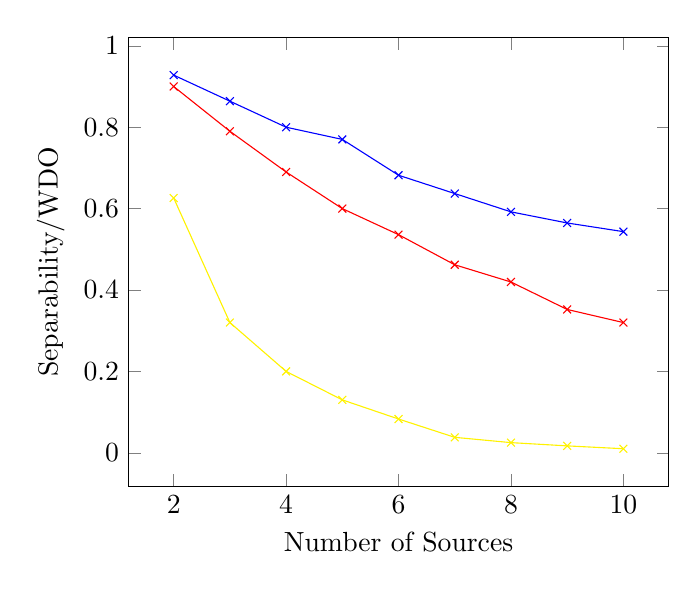
\begin{tikzpicture}
	\begin{axis}[
		xlabel=Number of Sources,
    ylabel=Separability/WDO]
    % speakers
	\addplot[color=red,mark=x] coordinates {
		(2,0.9)
		(3,0.79)
		(4,0.69)
		(5,0.6)
		(6,0.536)
		(7,0.462)
		(8,0.4197)
		(9,0.352199)
		(10,0.32)
  };
  % single note
  	\addplot[color=blue,mark=x] coordinates {
		(2,0.928)
		(3,0.864)
		(4,0.8)
		(5,0.77)
		(6,0.682)
		(7,0.637)
		(8,0.592)
		(9,0.5647)
		(10,0.5434)
  };
  % unison
    \addplot[color=yellow,mark=x] coordinates {
		(2,0.626)
		(3,0.32)
		(4,0.2)
		(5,0.13)
		(6,0.083)
		(7,0.038)
		(8,0.025)
		(9,0.017)
		(10,0.01)
	};
	\end{axis}
\end{tikzpicture}
\end{figure}

% TODO: add figure from google spreadsheets
% TODO: add little dataset table

\section{Real Mixtures}

Fundamental frequency estimation of a signal is a common task in audio signal processing with many applications. 
If the $F0$ varies over time, the complexity increases, and it is also more difficult to provide ground truth data for evaluation.
We therefore proposed a dataset targeted at high resolution ground truth information of the fundamental frequency variation of vibrato notes~\cite{stoeter15acm}.

\subsection{High Resolution Modulations}

\marginpar{This subsection is based on the work that has been published in~\cite{stoeter15acm} together with my former student Michael Müller who helped with the experiments.}

\begin{figure}[h]
  \centering
  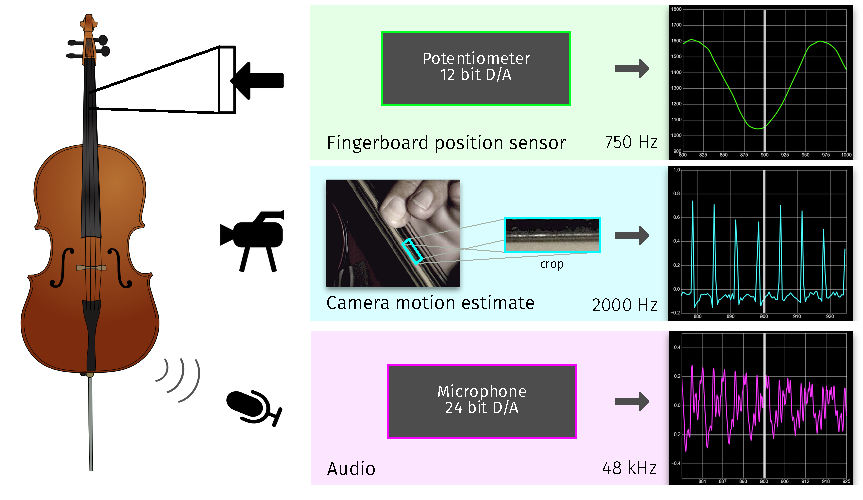
\includegraphics[width=\textwidth]{Chapters/04_Data/figures/teaser.pdf}
  \caption{Overview of the multi-modal data recorded for the proposed dataset.}
\label{fig:teaser}
\end{figure}

% from 
In turn, we included sensor recordings capturing the finger position on the fingerboard which is converted into an instantaneous frequency estimate. 
% TODO: provide further reference
In speech processing, the electroglottograph (EGG) is able to capture the excitation signal of the vocal tract, which is then used to generate a reference instantaneous $F0$.
Inspired by this, we included high speed video camera recordings to extract the excitation signal originating from the moving string.
In the proposed test set we chose the violin cello for the following reasons: (1) vibrato is used as a common style for expression, (2) there is an observable physical relationship between frequency modulation and vibrato, and (3) the instrument is large enough to embed sensors to capture the vibrato. The properties of the cello are studied by research in acoustics~\cite{woodhouse04, woodhouse99}.
The aim of the multi-sensor recordings is to capture major aspects of the cello while being played by a musician. We identify three main components: (1) Excitation caused by the moving bow; (2) the vibrating string, and (3) the finger, controlling the string length by rolling it on the fingerboard.
The main focus of the recordings is set to analyze vibrato playing style. Since it is common that vibrato characteristics differ from musician to musician, all recordings were performed by two musicians. One is a professional cellist with 30 years of experience in a symphonic orchestra. 
The other musician is an amateur, who has less than 1 hour per week of practice.
The recordings took place on a single day and were conducted on a mid-quality full-size cello equipped with sensors as described below. Due to the width of fingerboard sensors and the attached cables we were able to equip two strings (G and A) allowing to record pitches ${G2, D3, D^\sharp3, E3, A3, B3, C4, C^\sharp4}$ from both musicians. The resulting test set yields in $148$ recorded notes after removal of some notes due to errors in the sensor recordings. The process for cleaning up the data is documented\footnote{\url{https://github.com/audiolabs/muserc}}. The dataset is released under a Creative Commons license.

\subsection{Multitrack Data}

The Signal Separation Evaluation Campaign (SiSEC) is a solid indicator of the progress in research within the field of source separation \cite{vincent12}. The results from the last SiSECs show that for professionally produced music it is still difficult to achieve a high quality separation without using a significant amount of training data~\cite{sisec13, ono15, liutkus17, stoeter18sisec}.
Multitrack datasets are helpful to develop and evaluate methods on complex acoustic conditions.
% zaffar begin
Building a good data-driven method for source separation relies heavily on a training dataset to learn the separation model. In our case, this not only means obtaining a set of musical songs, but also their constitutive accompaniment and lead sources, summing up to the mixtures. For professionally-produced or recorded music, the separated sources are often either unavailable or private. Indeed, they are considered amongst the most precious assets of right holders, and it is very difficult to find isolated vocals and accompaniment of professional bands that are freely available for the research community to work on without copyright infringements.
% zafar end
\par
In the past years, datasets were proposed for many different source separation scenarios. We briefly describe the most important ones, summarized in Table~\ref{tab:datasets}. 

\begin{itemize}[leftmargin=*]
	\item The QUASI dataset was proposed to study the impact of different mixing scenarios on the separation quality. It  consists of the same tracks as in the MASS dataset, but kept full length and mixed by professional sound engineers.
	\item The MIR-1K and iKala datasets were the first attempts to scale vocals separation up. They feature a higher number of samples than the previously available datasets. However, they consist of mono signals of very short and amateur karaoke recordings.
	\item The ccMixter dataset was proposed as the first dataset to feature many full-length stereo tracks. Each one comes with a vocals and an accompaniment source. Although it is stereo, it often suffers from simplistic mixing of sources, making it unrealistic in some aspects.
	\item MedleyDB has been developed as a dataset to serve many purposes in music information retrieval. It consists of more than 100 full-length recordings, with all their constitutive sources. It is the first dataset to provide such a large amount of data to be used for audio separation research (more than 7 hours). Among all the material present in that dataset, 63 tracks feature singing voice.
  \item DSD100 was presented for SiSEC 2016. It features 100 full-length tracks originating from the 'Mixing Secret' Free Multitrack Download Library\footnote{\url{http://www.cambridge-mt.com/ms-mtk.htm}} of the Cambridge Music Technology, which is freely usable for research and educational purposes. An extended version, merging MedleyDB and DSD100 was recently released as MUSDB18~\cite{rafii17}
\end{itemize}

In any case, it can be seen that datasets of sufficient duration (see Table~\ref{tab:datasets}) to build data-driven separation methods were only created recently.

This package should nicely integrate with your existing python code, thus makes it easy to participate in the SISEC MUS tasks. The core of this package is calling a user-provided function that separates the mixtures from the DSD into several estimated target sources.

\begin{minted}{python}
import dsdtools

def my_function(track):
    estimates = {
        'vocals': track.audio,
        'accompaniment': track.audio,
    }
    return estimates

dsd = dsdtools.DB(root_dir="./Volumes/Data/dsdtools")
dsd.run(my_function, estimates_dir="path/to/estimates")
\end{minted}

% TODO: describe my own work here
TODO: add description of DSD100 tools
% TODO: Dataset parsers



% \begin{table*}[htbp]
% 	\centering
% 	\caption{Summary of datasets available for lead and accompaniment separation. Tracks without vocals were omitted in the statistics.}
% 	\label{tab:datasets}
% 		\begin{tabular}{l l l l l l}
% 			\hline
% 			\textbf{Dataset} & \textbf{Year} & \textbf{Reference(s)} & \textbf{Tracks} & \textbf{Track duration (s)} & \textbf{Full/stereo?}\\
% 			\hline
% 			MASS & 2008 & \cite{MTGMASSdb} & 9 & $16 \pm 7$ & no / yes \\
% 			MIR-1K & 2010 & \cite{hsu10} & 1,000 & $8 \pm 8$ & no / no \\
% 			QUASI & 2011 & \cite{liutkus11,vincent12} & 5 & $206 \pm 21$ & yes / yes \\
% 			ccMixter & 2014 & \cite{liutkus142} & 50 & $231 \pm 77 $ & yes / yes \\
% 			MedleyDB & 2014 & \cite{bittner14} & 63 & $206 \pm 121$ & yes / yes \\
% 			iKala & 2015 & \cite{chan15} & 206 & 30 & no / no \\
% 			DSD100 & 2015 & \cite{ono15} & 100 & $251 \pm 60$ & yes / yes \\
%       MUSDB18 & 2017 & \cite{rafii17} & 150 & $236 \pm 95$ & yes / yes \\
% 			\hline
% 		\end{tabular}
% \end{table*}

